\documentclass{standalone}\usepackage[]{graphicx}\usepackage[]{color}
%% maxwidth is the original width if it is less than linewidth
%% otherwise use linewidth (to make sure the graphics do not exceed the margin)
\makeatletter
\def\maxwidth{ %
  \ifdim\Gin@nat@width>\linewidth
    \linewidth
  \else
    \Gin@nat@width
  \fi
}
\makeatother

\definecolor{fgcolor}{rgb}{0.345, 0.345, 0.345}
\newcommand{\hlnum}[1]{\textcolor[rgb]{0.686,0.059,0.569}{#1}}%
\newcommand{\hlstr}[1]{\textcolor[rgb]{0.192,0.494,0.8}{#1}}%
\newcommand{\hlcom}[1]{\textcolor[rgb]{0.678,0.584,0.686}{\textit{#1}}}%
\newcommand{\hlopt}[1]{\textcolor[rgb]{0,0,0}{#1}}%
\newcommand{\hlstd}[1]{\textcolor[rgb]{0.345,0.345,0.345}{#1}}%
\newcommand{\hlkwa}[1]{\textcolor[rgb]{0.161,0.373,0.58}{\textbf{#1}}}%
\newcommand{\hlkwb}[1]{\textcolor[rgb]{0.69,0.353,0.396}{#1}}%
\newcommand{\hlkwc}[1]{\textcolor[rgb]{0.333,0.667,0.333}{#1}}%
\newcommand{\hlkwd}[1]{\textcolor[rgb]{0.737,0.353,0.396}{\textbf{#1}}}%

\usepackage{framed}
\makeatletter
\newenvironment{kframe}{%
 \def\at@end@of@kframe{}%
 \ifinner\ifhmode%
  \def\at@end@of@kframe{\end{minipage}}%
  \begin{minipage}{\columnwidth}%
 \fi\fi%
 \def\FrameCommand##1{\hskip\@totalleftmargin \hskip-\fboxsep
 \colorbox{shadecolor}{##1}\hskip-\fboxsep
     % There is no \\@totalrightmargin, so:
     \hskip-\linewidth \hskip-\@totalleftmargin \hskip\columnwidth}%
 \MakeFramed {\advance\hsize-\width
   \@totalleftmargin\z@ \linewidth\hsize
   \@setminipage}}%
 {\par\unskip\endMakeFramed%
 \at@end@of@kframe}
\makeatother

\definecolor{shadecolor}{rgb}{.97, .97, .97}
\definecolor{messagecolor}{rgb}{0, 0, 0}
\definecolor{warningcolor}{rgb}{1, 0, 1}
\definecolor{errorcolor}{rgb}{1, 0, 0}
\newenvironment{knitrout}{}{} % an empty environment to be redefined in TeX

\usepackage{alltt}
\usepackage{tikz}
\IfFileExists{upquote.sty}{\usepackage{upquote}}{}
\begin{document}
 
 
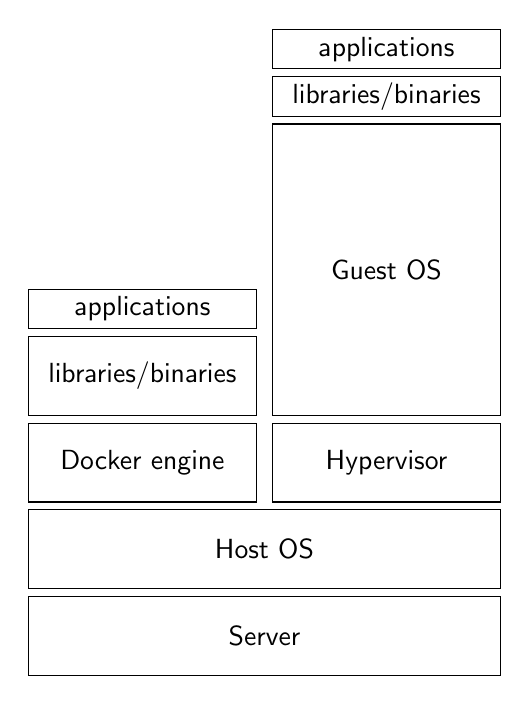
\begin{tikzpicture}
font=\sffamily
%% three long rects for server, host OS, hypervisor/docker engine
\draw (0,0) rectangle (6,1) node[midway] {Server};
\draw (0,1.1) rectangle (6,2.1) node[midway] {Host OS};
%% side by side rects for hypervisor/docker engine
\draw (0,2.2) rectangle (2.9,3.2) node[midway] {Docker engine};
\draw (3.1,2.2) rectangle (6,3.2) node[midway] {Hypervisor};
%% side by side rects for VM OS / shared bins libs
\draw (0,3.3) rectangle (2.9,4.3) node[midway] {libraries/binaries};
\draw (3.1,3.3) rectangle (6,7) node[midway] {Guest OS};
%% side by side rects for shared bins libs
\draw (0,4.4) rectangle (2.9,4.9) node[midway] {applications};
\draw (3.1,7.1) rectangle (6,7.6) node[midway] {libraries/binaries};
%% side by side rect for VM app
\draw (3.1,7.7) rectangle (6,8.2) node[midway] {applications};
 
 
\end{tikzpicture}
 
 
\end{document}
